\chapter{Results} \label{chapterResults}

% Results, findings, discussion of results OR manuscripts. It is best to reiterate information in your literature review to help substantiate your research findings.

With our narrowed focus on repositories, we can now spend more time looking through the data collected. Specifically, we gathered data on the Refactor Warnings provided by Pylint. In Table \ref{table:smallRefactorWarningTotals} we have a shortened listing of the repositories from our set with their total count of refactoring warning messages, in addition to the most commonly appearing to refactor warning message. For the entire set, see Table \ref{table:allRefactorWarningTotals} in the Appendix.

\begin{table}[ht]
  \small
  \centering
  \begin{tabularx}{0.8\textwidth} {
    | l 
    | c
    | >{\centering\arraybackslash}X 
    | c |
  }
    \hline
    Repository Name & Msg Count & Top Msg & Top Msg Count \\
    \hline\hline
    sympy & 14,206 & too-many-arguments & 6,601 (46\%) \\ \hline
    ansible &  10,431 & no-else-return & 1,711 (16\%) \\ \hline
    salt &  7,814 & too-many-arguments & 1,640 (21\%) \\ \hline \hline
    ranger & 109 & no-else-return & 29 (27\%) \\ \hline
    sentry & 66 & no-self-use & 32 (48\%) \\ \hline
    raven-python & 20 & too-few-public-methods & 7 (35\%) \\ \hline
  \end{tabularx}
  \caption{Total refactor messages per repository for the 3 best and 3 worst offendors. Also provided with the refactor message that had the most warnings and its total count (and the percentage of that message from the total refactor warnings for that repository).}
  \label{table:smallRefactorWarningTotals}
\end{table}

Regarding the number of refactoring warning messages, we can see that the ``worst'' project in our set was the repository Sympy \cite{data:sympy}, with 14,206 refactor messages. However, project size may also weigh how many warnings and errors are present, as projects with more lines of code are presumed to have more errors.

If we instead look at the ratio of refactoring warnings to the total lines of source code, we get a very different picture, provided in Table \ref{table:smallRefactorSLOCRatio}. We calculated these values using the following equation, $r$ is the total refactor message count for the project, $c$ is the total number of source lines of code in the project, and 100 is a multiplier to make the numbers easier to wrap our heads around. So the numbers closer to 0 are better ratios, as there are fewer refactor messages in the project relative to its size.

$$
Refactor \space Ratio = r / c * 100
$$

In this case, the repository Raven-Python \cite{data:raven-python} (which was the ``best'' in regards to total refactor message count) is now the ``worst'' with the highest ratio of refactoring warnings compared to the lines of source code in the project. Raven-Python also has the least count of SLOC in the entire repository set!

\begin{table}[ht]
  \small
  \centering
  \begin{tabularx}{1.0\textwidth} {
    | l 
    | r
    | r
    | >{\centering\arraybackslash}X |
  }
    \hline
    Repository & Total Refactor Msgs & Total Project SLOC & Ratio \\
    \hline\hline
    raven-python & 20 & 1,474 & 1.35 \\ \hline
    scrapy & 381 & 58,768 & 0.64 \\ \hline
    numba & 126 & 20,192 & 0.62 \\ \hline \hline
    electrum & 722 & 425,576 & 0.16 \\ \hline
    youtube-dl & 1,003 & 667,075 & 0.15 \\ \hline
    cython & 1,718 & 1,183,863 & 0.14 \\ \hline
  \end{tabularx}
  \caption{Total refactor messages per repository, total project source line of code (SLOC), and the ratio of refactor messages to SLOC.}
  \label{table:smallRefactorSLOCRatio}
\end{table}

Given that we now have an idea of which projects have the most refactor messages per line of source code (``worst'' offenders) and the projects with the least refactor messages (``best'' projects for maintainability), we can look a little closer at the most frequent messages. For example, common to all six repositories at a high frequency is the message ``no-self-use'' and ``no-else-return''. The message ``no-self-use'' means that `self' is used as an argument but not in the method; this should be handled differently. For example, the message ``no-else-return'' highlights when an unnecessary code block follows an if-conditional.

Some of the other common messages call out the use of ``too many'' of different types of objects. For example, ``too-many-branches'', ``too-many-arguments'', ``too-many-locals'', ``too-many-statements''... 

\vspace{0.25cm}
\begin{displayquote}
  ``Software maintainability these days has become one of the essential external attributes of software, which further forms a basis of research for many researchers working in the fields related to software engineering. Software maintainability can be described as how a particular software system can be changed concerning the number of Lines of Code (LOC).'' \cite{gupta:2021}
\end{displayquote}
\vspace{0.25cm}

Now, it would be helpful to understand where we stand on the Maintainability Index (MI) for these projects, as this is our form of measurement that will help us understand how the code might be able to evolve. The MI is calculated on a per-module basis, but for the sake of conversation (and acknowledging that we will lose some nuances by reducing it this way), let us find the average MI at the project level and add this to our table (Table \ref{table:smallRefactorSLOCRatio2}). Also included is the standard deviation for each average, with the lowest standard deviation being 13.75 and the highest at 31.14. Most averages have a standard deviation between 20 and 30 points.

\begin{table}[ht]
  \small
  \centering
  \begin{tabularx}{1.0\textwidth} {
    | l 
    | r
    | r
    | r
    | >{\centering\arraybackslash}X |
  }
    \hline
    Repo & Refactor Msgs & Project SLOC & Ratio & Avg Project MI \\
    \hline\hline
    raven-python & 20 & 1474 & 1.35 & 87.02 ±13.75 \\ \hline
    scrapy & 381 & 58768 & 0.64 & 64.47 ±17.72 \\ \hline
    numba & 126 & 20192 & 0.62 & 62.55 ±21.08 \\ \hline \hline
    electrum & 722 & 425576 & 0.16 & 39.41 ±28.06 \\ \hline
    youtube-dl & 1003 & 667075 & 0.15 & 54.16 ±19.95 \\ \hline
    cython & 1718 & 1183863 & 0.14 & 31.02 ±29.19 \\ \hline
  \end{tabularx}
  \caption{Total refactor messages per repository, total project source line of code (SLOC), the ratio of refactor messages to SLOC, average Maintainability Index (MI).}
  \label{table:smallRefactorSLOCRatio2}
\end{table}

\todo{With our more minor data set on hand, we ran Radon against each repository to gain a Maintainability Index. We averaged the Maintainability Index of all files within each project for a very simplified view. This gave us a single number for general comparison with each repository.}

\todo{The ``Avg MI'' column in the table contains the calculated average value for each file in the project. In Radon's grading system, any value over 20 is considered a ``very maintainable'' code. We also used a count of the Pylint REFACTOR messages and calculated the ratio of messages to source-line-of-code for how many code smells each project contained relative to its size. This calculated ratio is shown in the ``Ratio'' column. Listed in the table are the ``best 3'' (cython, youtube-dl, and electrum) and the ``worst 3'' (raven-python, scrapy, and numba) regarding their refactor ratios.}

When reviewing the Maintainability Inde for our repositories at either end of the spectrum and in context with the entire set (see Appendix \ref{table:allRefactorSLOCRatio}), we will find that while Raven-Python has the highest number of refactoring warnings when compared to the SLOC count. Raven-Python also has the second-highest average MI across all of its project files.

Of the entire set, our highest average MI is 87.38 ±19.47 (belonging to Sentry), and our lowest average MI is 28.85 ±27.37 (belonging to MatPlotLib). Regardless, these average values are above a score of 20, which is Radon's lowest score provided for an ``A'' rank, that is, what would be considered a project ``very high'' maintainability.

With this information, we can get an idea of where these projects stand regarding their refactor message ratios compared to each other. For example, the histogram in Fig. \ref{figHistogramRefactorRatio} shows that the majority of our repository set has a meager ratio of refactoring messages. However, the mass projects on the low-end could indicate that our projects are highly maintainable based on our assumptions that refactor messages are related to maintainability. Having few refactor messages (relative to the number of lines of code) means we have a smaller number of code smells. Therefore, infrequent refactor warnings are helpful for our architecture and quality!

\begin{figure}[ht]
  \centerline{
    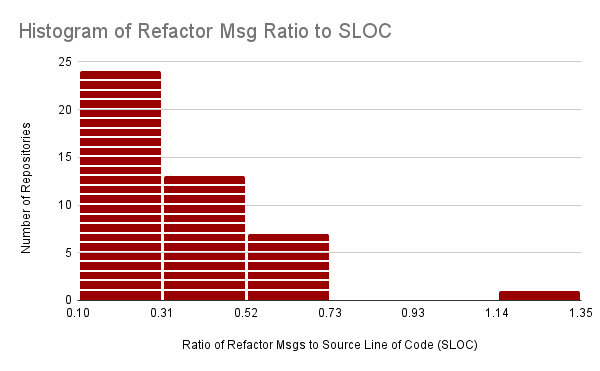
\includegraphics[width=0.8\columnwidth]{Histogram of Refactor Msg Ratio to SLOC.png}
  }
  \caption{Histogram of the number of refactor messages relative to the size of the project as measured by source lines of code. Diligent development communities can keep refactor warnings low, regardless of system size (lines of code).}
  \label{figHistogramRefactorRatio}
\end{figure}

The data set we chose may impact the ratios, lending to them all being on the low end. Perhaps open-source projects with highly engaged communities tend to keep their code in a maintainable state because this would be the only way for significant involvement (over 90 contributors per project). It has been interesting to see how low the ratio of refactoring messages has been in our data set.

To view the same repository set with their Maintainability Index averages, we have another histogram in Fig. \ref{figHistogramAvgMI}. This Radon score can range from 0 (awful) to 100 (perfect). Radon considers any value above 20 to be an ``A'' or ``very maintainable''. All of our projects receive an ``A'' grade, with the majority in the middle range (around 40 to 50). All projects in our data set were all mid-to high-range scores.

\begin{figure}[ht]
  \centerline{
    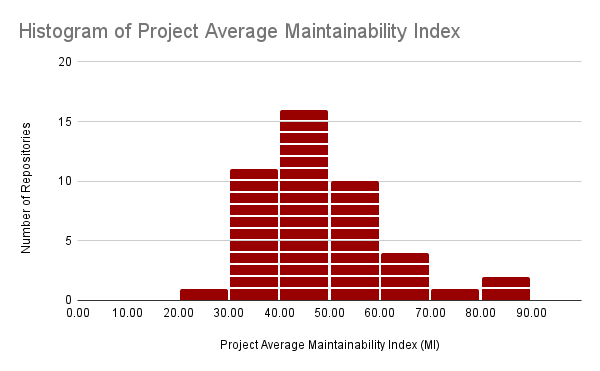
\includegraphics[width=0.8\columnwidth]{Histogram of Project Average Maintainability Index_BucketSize_10.png}
  }
  \caption{Historgram of project average Maintainability Index (MI).}
  \label{figHistogramAvgMI}
\end{figure}
